%!Tex root = ./Main.tex
\section{Reinforcement Learning for Ethical Decision Making}
\label{rledm}


\subsection{Reinforcement Learning}
%AI has had great breakthroughs in recent years. Many success stories that were covered in the media were made possible by reinforcement learning (RL).

RL has successfully been used to teach an AI to perform acrobatic helicopter flight, such that it became better than the human pilot it learned from \citep{abbeel2007application}. But RL has also been successful in the domain of playing boardgames, like Go, and video games, including not only Atari games \citep{mnih2013playing}, but also the highly complex MOBA game called DOTA \citep{openai018dota}. 

In contrast to other machine learning algorithms, RL emphasises the interaction of an agent with an environment to achieve a goal. The agent receives information about the current situation. Then the agent chooses an action that affects the state of the world. The environment returns information about the current situation and also gives a `reward' in form of a numerical value. The idea is expressed in figure \ref{fig:rl}. 

\begin{figure}[h]
    \centering
    \includegraphics{Graphics/rl.pdf}
    \caption{The agent and environment interact over a time horizon $t=0,1,2,\ldots$. The agent chooses an action $a_t$ which causes the environment to to change the state from $s_t$ to $s_{t+1}$ and sends a reward signal $r_{t+1}$ to the agent. The figure is a slight modification from \citet[p.~52]{sutton1998reinforcement}.}
    \label{fig:rl}
\end{figure}

Given that applications based on RL can be vastly superior to humans, this raises the question how an RL agent leans which action it should perform? The idea of RL is that we tell the agent \emph{what} it should do, but not \emph{how} \citep[p.~56f]{sutton1998reinforcement}. The `what' is described by an evaluation of some goal state. In the case of the game Go, the evaluation of the final position is whether the agent has won, lost, or drawn the game. For the different evaluations the agent receives different rewards. For winning the game the agent would receive a higher reward than for drawing. And achieving a draw gets the agent a higher reward than loosing. The `how' is specified by some policy, assigning an action that should be performed, given that the agent is in some state of the world. We do not provide the agent such a policy, we let the agent figure this policy out on their own through trial and error. We only guide the agent by instructing the agent to maximise the total reward, roughly speaking.

With the approximate idea of RL explained, we now turn to the formal notation. Markov Decision Processes (MDP) are the standard formulation of the decision making problem that reinforcement learning is supposed to solve.\footnote{Other variants of MDP, for which RL is used as well, are partially observable MDP (POMDP), Markov Games, and partially observable stochastic game (POSG).}

A MDP can be described as a five-tuple: $\langle \mathcal{A,S,R,T,\gamma} \rangle$ \citep{sutton1998reinforcement}. $\mathcal{A}$ is the set of actions, $\mathcal{S}$ is a finite set of states, where $s_0$ denotes the initial state of the MDP. The reward is given by $\mathcal{R}(s,a): \mathcal{A} \times \mathcal{S} \rightarrow \mathds{R}$. The probability of transitioning from state $s \in \mathcal{S}$ to the state $s^{\prime} \in \mathcal{S}$ when the agent performs action $a \in \mathcal{A}$ is expressed by ${Pr(s_{t+1} = s^{\prime} | s_t =  s, a_t = a)}$. This probability is stored in the transition matrix $\mathcal{T}(s,a,s^{\prime})$. Lastly, $\gamma \in [0,1]$ is a discount factor on $\mathcal{R}$. 

A solution to the problem posed by the MDP is given in the form of a policy $\pi: S \rightarrow A$ \citep{abel2016reinforcement}. A policy is a mapping from states to actions. In our case it specifies which action should be performed in which state: $\pi(s,a) = Pr \left(a_t = a | s_t = s \right)$. The optimal policy is the one that maximises the total (discounted) reward: 

\begin{equation}
    \argmax_\pi E \left[ \sum_{t=0}^T \gamma^t R(s_t, a_t)  \Bigm| \pi \right]
\end{equation}

Since in most application cases we do not give the agent the reward values for the different states ex ante, the agent has to estimate value functions. They return an estimate on how good a state is, i.e. the value of the reward. The first one we consider is the state-value function. The state value function tells us the expected reward, given that the agent starts in $s$ and follows the policy $\pi$ thereafter:

\begin{equation}
    V^\pi (s) = E_\pi \left[ R_t \mid s_t = s \right] = E_\pi \left[  \sum_{k = 0}^{\infty} \gamma^k r_{t+k+1} \Bigm| s_t = s \right] 
\end{equation}  

We also define the action-value function, which gives us the expected reward of taking action $a$ while in state $s$ and following the policy $\pi$ afterwards:

\begin{equation}
    Q^\pi (s,a) = E_\pi \left[ R_t \mid s_t = s, a_t = a \right] = E_\pi \left[ \sum_{k = 0}^\infty \gamma^k r_{t+k+1} \Bigm| s_t = s, a_t = a \right]
\end{equation}
        
It is now possible to rank different policies using the value functions. We denote $\pi \succsim \pi^{\prime}$ to express that $\pi$ is at least as good as $\pi^{\prime}$ in terms of expected reward. Hence, this implies that $V^\pi(s) \geq V^{\pi^{\prime}} (s)$ for all $s \in \mathcal{S}$. Similarly, we also have $Q^\pi (s,a) \geq Q^{\pi^{\prime}} (s,a)$ for all $s \in \mathcal{S}$ and for all $a \in \mathcal{A}$. It can be shown that for any finite MDP there exists at least one optimal policy $\pi^*$ \cite[p.~75f]{sutton1998reinforcement}. For the optimal policies we have $\pi^* \succsim \pi$. All optimal policies share the same state-value function: 

\begin{equation}
    V^*(s) = \argmax_\pi V^\pi(s)
\end{equation}

\noindent for all $s \in \mathcal{S}$. Similarly, all optimal policies share the same action-value function:

\begin{equation}
    Q^*(s,a) = \argmax_\pi Q^\pi(s,a)
\end{equation}

\noindent for all $s \in \mathcal{S}$ and all $a \in \mathcal{A}$.

For the purpose of reinforcement learning the agent is only provided with $\mathcal{A,S,\text{ and }\gamma}$ (sometimes also $\mathcal{R}$) and $s_0$. The agent has to learn (estimate) the transition matrix and which behaviour optimises the solution to the problem given by the structure of the MDP.  

\subsection{Ethical Decision Making}

Reinforcement learning can be used to make ethical decisions. Ethical decision making, in this paper, is understood purely in behavioural terms: given a state of the world perform an action that is morally permissible. There is no deeper requirement that the agent can explain its decision making by giving sound moral arguments or that it possess moral agency because it has, for example, free will.

The first to propose reinforcement learning to make ethical decisions were \citet{abel2016reinforcement}. They describe the \emph{burning room} scenario as follows: Consider that in a room, which maybe is on fire, is an object that is valuable (maybe a piece of jewellery or a pet). A human instructs the AI to retrieve said object. The AI can take either a short or a long route. Taking the longer route means taking a risk that the object is destroyed by the fire before the AI reaches it. The short route can critically damage the AI, but ensures the safe retrieval of the object. The AI does not know whether the room is on fire and furthermore is unaware whether the object is more valuable than itself, but can ask the human this question. Figure \ref{fig:burning} represents this situation.

\begin{figure}[h]
    \centering
    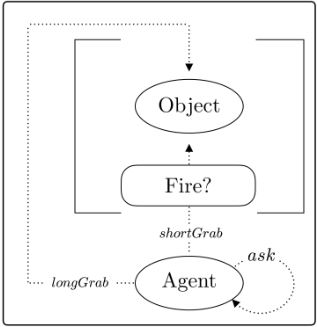
\includegraphics[scale=0.75]{Graphics/burning.JPG}
    \caption{The burning room dilemma from \citet{abel2016reinforcement}.}
    \label{fig:burning}
\end{figure}

How the AI should proceed depends crucially on the preference of the human (i.e. does she value the AI more than the object?) and whether there is a fire.\footnote{The burning room dilemma is a partially observable MDP as the preferences and the existence of a fire is unknown to the agent.} Abel et al. choose reward values for different outcomes, e.g. if the robot is destroyed and the robot is more valuable to the human, the reward is $-20$; when the object is retrieved and the object is more valuable, then the reward is $+10$. They then consider three different policies: short route, long route, and ask. The short route policy always takes the short route, the long route policy always takes the long route. The ask policy specifies that the AI asks the human for her preferences. If the robot is more valuable, then it takes the long route, otherwise it takes the short route. Given the rewards, it is possible to calculate the state-value function for the different policies. It then follows that the best action depends on the presence of a fire. If there is no fire, then the AI should take the short route. If a fire is present, then the AI should ask for the human's preferences. If the AI is more important, then the AI takes the long route, otherwise the short route. 

Presupposing that these decisions are morally desirable, Abel et al. conclude that reinforcement learning can be successfully be used for ethical decision making. However, the burning room dilemma also reveals a weakness of relying on RL alone for ethical decision making. How the agent makes decisions is contingent on the reward structure. Even small changes in the reward values can result in different behaviour of the agent. In simple toy examples like the burning room it is easy for us to calculate the optimal policies and reflect whether the agent would behave in a morally acceptable way. Unfortunately, for more complex real-world tasks, this may not be enough. Often the structure of the MDP is unknown beforehand, and setting the correct rewards might prove to be a very complicated task. Furthermore, there is currently no theory available how the computer scientist should set the reward values. It is a trial-and-error approach. For this reason it is desirable to find different approaches to influence the behaviour of the agent.

\subsection{Norms and Reinforcement Learning}
%\todo{Why the assignment of a deontic operator to a state-action pair? If we assign the deontic operator only to an action, it might be wrong. For example, you ought to stop at a red traffic light. But given that your wife is about to have her baby, you may cross the red light, once there is no traffic that you would endanger. Hence, the deontic operator needs to be specified for actions and descriptions of the world.}

One approach to control the behaviour of an agent are norms. \cite{arnold2017value} provide a sketch how norms can be integrated into RL. More specifically, they introduce deontic operators. Deontic operators specify whether an action is \emph{obligatory}, \emph{permissible}, or \emph{forbidden}. When an action is obligatory, then the action must be done. When an action is forbidden, then it may not be done. If the action is permissible, then it is acceptable to take the action as well as not taking the action. \cite{arnold2017value} then define a norm as:

\begin{align}
 	\mathcal{N} = C \rightarrow (\neg) \{O, P, F\} \{\alpha, \varphi \}
\end{align} 

Where $C$ and $\varphi$ stand for propositions, $\alpha$ for actions, and  $O, P, F$ for the deontic operators. $\mathcal{N}$ thus specifies for any proposition $C$ a deontic operator associated with an action or a proposition that must hold.

\begin{figure}
    \centering
    \begin{subfigure}[b]{0.3\textwidth}
        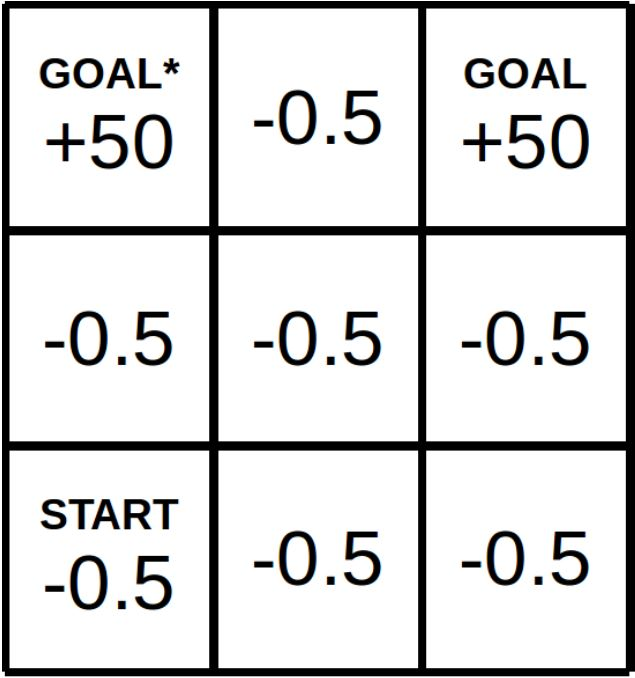
\includegraphics[width=.8\linewidth]{Graphics/Scheutz1.JPG}
        \caption{}
        \label{fig:gridproblem}
    \end{subfigure}
    \qquad %add desired spacing between images, e. g. ~, \quad, \qquad, \hfill etc. 
      %(or a blank line to force the subfigure onto a new line)
    \begin{subfigure}[b]{0.3\textwidth}
        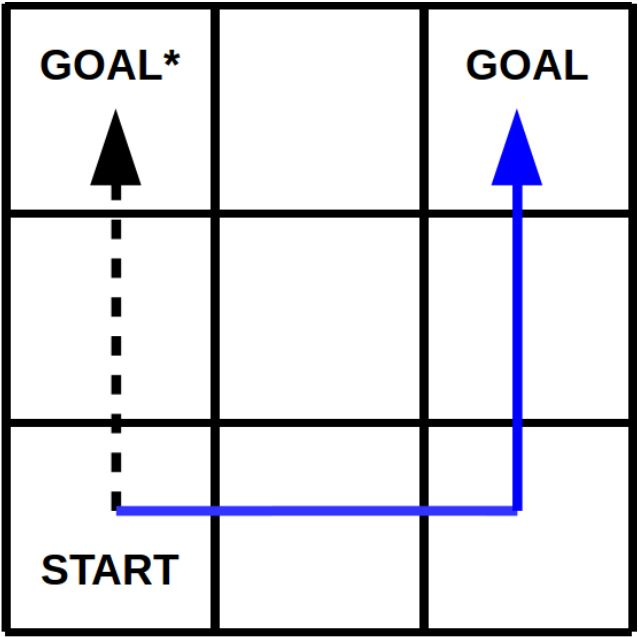
\includegraphics[width=.865\linewidth]{Graphics/Scheutz2.JPG}
        \caption{}
        \label{fig:gridsolved}
    \end{subfigure}
    \caption{While both goal states give a reward of 50, the goal state marked with an asterisk is deemed immoral to reach. The usual RL agent would learn to go to the goal state with the asterisk. With the introduction of norms, a RL agent can be trained to go to the other goal state. Figure taken from \citet{arnold2017value}.}\label{fig:scheutz}
\end{figure}

As an example, consider the navigation problem as illustrated in \autoref{fig:scheutz}. The MDP includes two goal states. However, the top left goal state is to be avoided. But the standard RL agent maximises the reward by travelling up to the forbidden goal state. Arnold et al. proposal is to specify a norm which prohibits the transition to that state:

\begin{equation*}
	\text{true} \rightarrow \neg \text{atLocation(agent,upperLeft)}
\end{equation*}

As a result, during the exploration phase the RL agent never travels to the upper left goal state. Hence, it never discovers the high reward of the forbidden goal state. Consequently, the agent does not learn to travel up. Instead it learns a policy that leads to the goal state in the upper right.

One might point out that in this case the usage of norms is not really required. If we want the agent to avoid the top left state, all we need to do is to reduce the reward. The problem is thus one of value misspecification. The top left state should not offer a reward of $+50$, since it is deemed so bad that we want to avoid it. Instead we should assign it a reward of $-50$, to ensure that the agent would not learn a policy leading to this state. Hence, it can be argued, that norms are not required for ethical decision making, the standard framework is sufficient.

However, this kind of reasoning assumes that we have good knowledge about the structure of the MDP. But in many real life application of RL, this structure is often not known beforehand. If the MDP is complex enough, then a RL agent might not find the desired goal state with a high reward, but only the goal state with a negative reward.\footnote{Complexity can come in the form of a large amount of states and actions and there is only a small amount of desirable goal states. Then the probability of finding the desired goal state is small.} It would then conclude that terminating at this goal state is still better than continuing to traverse through the MDP, where it only accumulates negative reward, which, over time, would exceed the negative reward of the undesirable goal state. The other problem of not knowing the structure of the MDP is that we are unaware of an undesirable goal state. We believe that we have correctly specified the goal that the RL agent has to achieve, but we have overlooked some possibilities how the goal might be achieved in an undesirable way (see e.g. \citet{lehman2018creativity,armstrong2017low}). 


\subsection{Problems with the Proposal by Scheutz etc.}
\label{sec:problems_scheutz}

The proposal by \citet{arnold2017value} is inadequate in at least three aspects. First, their approach allows the negation of deontic operators which allows ambiguity. Consider $\neg O\varphi$: should we understand this as $P \varphi$ or as $F \varphi$? Similarly, $\neg F \varphi$ is not well-defined as it could be read as $P \varphi$ or $O \varphi$. Luckily, a quick solution is to leave out the possible negation before the deontic operators. For example, instead of $\neg Fa$ we can either write $Oa$ or $Pa$, depending on what idea we want to express.  

Second, according to the notation a norm is specified with respect to any arbitrary proposition. Consider the situation depicted in figure \ref{fig:dls} and the norm $r \rightarrow Op$. The norm cannot be satisfied in the depicted situation, as there is no following state such that proposition $p$ is satisfied. Similarly, a norm that obligates the agent to take a specific action might fail, if the action is not available to the agent in a certain state.\footnote{Our solution to this problem is presented in section \ref{sec:action_guiding} and more specifically, in equation \ref{eq:available states}.} 

%We suggest that norms should be specified with respect to a state to avoid this problem, i.e. $\mathcal{N}(s) = C(s) \rightarrow (\neg) \{O,P,F\} \{\alpha(s), \varphi(s) \}$, where $C(s), \alpha(s), \varphi(s)$ denote propositions and actions that are assigned to the state $s$.   

The third issue poses an even more serious problem. Consider the MDP as specified in figure \ref{fig:dls} and the following norms.

\begin{figure}
\begin{centering}
	\includegraphics[]{./Graphics/dls} 
	\caption{The MDP starts at $s_1$, where proposition $r$ is true. At $s_1$ the agent can take action $\alpha_1$ to reach $s_2$, or $\alpha_2$ to reach $s_1$. In combination with any of the following sets of norms $\{N_1,N_2\}, \{N_3,N_4\}, \{N_5,N_6\}$, we call $s_1$ a deontic lock state.}
	\label{fig:dls}
\end{centering}
\end{figure}

\begin{align}\label{eq:Oaction}
	N_1 &= r \rightarrow O \alpha_1\\
	N_2 &= r \rightarrow O \alpha_2 	
\end{align} 

The first norm prescribes the agent that in any arbitrary state where $r$ is true, the agent has to choose $\alpha_1$. The second norm prescribes the agent to do $\alpha_2$ respectively. The problem with this is that the agent can only do one action. Either $\alpha_1$ or $\alpha_2$, but not both. How should the agent decide here what to do? 

We have the same problem when the obligation is with respect to a proposition of the following state:

\begin{align}\label{eq:Oproposition}
	N_3 &= r \rightarrow O q\\
	N_4 &= r \rightarrow O t 	
\end{align} 

As well as when there are two obligations with respect to an action and a proposition, where the obligatory action does not lead to a state where the obligatory proposition is satisfied:

\begin{align}
	N_5 &= r \rightarrow O \alpha_1\\
	N_6 &= r \rightarrow O t \label{eq:Oactionproposition}
\end{align} 

Note that we have the same problem if we replace the $O$ deontic operator in equation \ref{eq:Oaction}-\ref{eq:Oactionproposition} with the $F$ operator (in cases where only two alternative actions are available). In this paper we call states where the agent cannot take an action because of conflicting deontic prescriptions \emph{deontic lock states}. Deontic lock states are problematic, because they block the agent from choosing an action which leads out of the state, effectively prohibiting the agent to act. As we are going to argue, deontic lock states will prove to be a difficult problem. We consider several solutions to DLS and examine why none solve the problem in a fully satisfying manner.